\appendix

\chapter{Comparativo de preços}

\begin{table}[!htpb]
 \centering
    \begin{tabular}{|p{4cm}|p{2cm}|p{4cm}|p{4cm}|} 
    \hline
        \textbf{Periféricos} & \textbf{Preço} & \textbf{Sistema Computacional com \textit{Raspberry Pi}} & \textbf{Sistema Computacional com \textit{desktop}} \\
    \hline
        Monitor c/ entrada HDMI & R\$ 404,10 & X & X \\
    \hline
        Cabo HDMI & R\$ 14,90 & X & X \\
    \hline
        Mouse USB & R\$ 9,99 & X & \\
    \hline
        Teclado USB & R\$ 22,40 & X & \\
    \hline
        Cartão MicroSD 8GB com adaptador & R\$ 32,52 & X & \\
    \hline
        Carregador Micro USB (fonte de alimentação) & R\$ 39,90 & X & \\
    \hline
        Cabo de força (fonte de alimentação) & R\$ 5,30 & & X \\
    \hline
        Placa \textit{Raspberry Pi} & R\$ 176,02 & X & \\
    \hline
        \textit{Desktop} (mouse e teclado inclusos) & R\$ 719,10 & & X \\
    \hline
        \textbf{TOTAL} & & \textbf{R\$ 699,83} & \textbf{R\$ 1.143,40} \\
    \hline
    \end{tabular}
    \caption{Comparativo entre sistemas computacionais}
    \label{t_fixa}
\end{table}

\chapter{Questionário}

\begin{figure}[ht]
    \centering
    \scalebox{0.4}{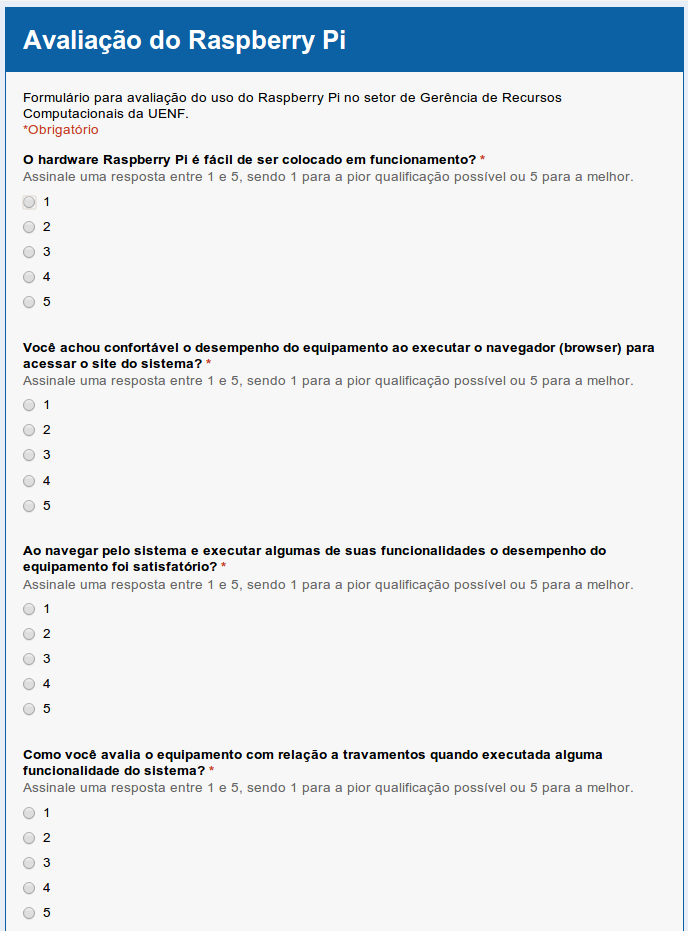
\includegraphics{figuras/questionario1}}
    \caption{Primeira parte do questionário}
\end{figure}

\begin{figure}[ht]
    \centering
    \scalebox{0.4}{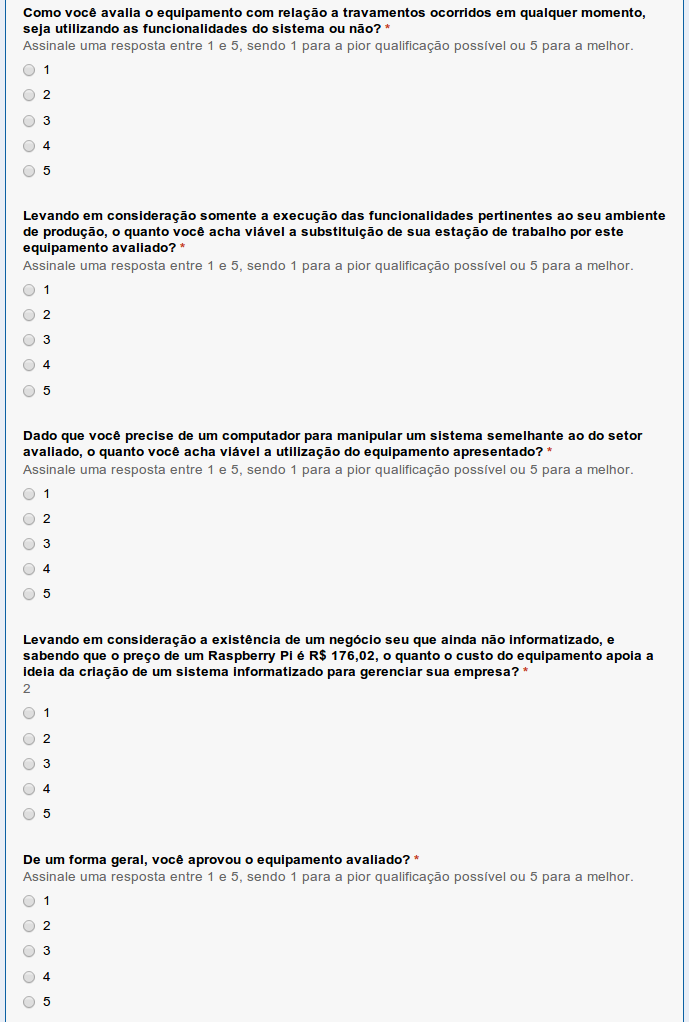
\includegraphics{figuras/questionario2}}
    \caption{Segunda parte do questionário}
\end{figure}